%%\documentclass[12pt]{article}
\documentclass[12pt]{elsarticle}
\usepackage{graphicx}
\usepackage{subfig}
\usepackage{amssymb,hyperref,rotating}
%\usepackage{draftwatermark}
%\SetWatermarkScale{2.0}
%\usepackage{dcolumn}
%\usepackage{bm}
%\documentstyle{psfig,epsf}{article}
%\usepackage{psfig,wrapfig,floatfig,float}
%\topmargin 0.5cm
%\addtolength{\evensidemargin}{-1.5cm}
%\addtolength{\oddsidemargin}{-1.5cm}
%\addtolength{\textwidth}{2.54cm}
%\addtolength{\topmargin}{-1.5cm}
%\addtolength{\textheight}{2.54cm}

\topmargin=-0.25in
\textwidth=6.25in
\textheight=8.25in
%\textheight=9.25in
\oddsidemargin=0.125in
\evensidemargin=0.125in

%\addtolength{\textwidth}{1.2in}
%\addtolength{\topmargin}{-.7in}
%\addtolength{\leftmargin}{-1.1in}
%\addtolength{\footskip}{-1.5cm}
%%\setlength{\textheight}{9.25in}
%\setlength{\textheight}{9.3in}
%%\setlength{\parindent}{1em}
%\setlength{\parskip}{1ex}
%%\pagestyle{headings}
%\setlength{\oddsidemargin}{0.in}
%\setlength{\evensidemargin}{0.in}
%\renewcommand{\thepage}{Eric D. Church/page \arabic{page}}
\thispagestyle{empty}

\pagestyle{myheadings}
\begin{document}
\title{The Liquid Argon Offline Software Package: LArSoft} 
\author{Jonathan Asaadi}
\address{}
\ead{}
\author{Bruce Baller}
\address{}
\ead{}
\author{Ben Carls}
\address{}
\ead{}

\author{Eric Church}
\address{Yale University, PO Box 500, MS309, Fermi National Accelerator Lab, Batavia, IL, USA, 60510-5011}
\ead{echurch@fnal.gov}
\author{Bonnie Fleming}
\address{Yale University, PO Box XYZ, Physics Department, Yale University, New Haven, CT, USA, 12345-1234}
\ead{bonnie.fleming@yale.edu}
\author{Herb Greenlee}
\address{}
\ead{}
\author{Ben Jones}
\address{}
\ead{}
\author{Wes Ketchum}
\address{}
\ead{}
\author{Brian Rebel}
\address{PO Box XYZ, MS309, Fermi National Accelerator Lab, Batavia, IL, USA, 60510-5011}
\ead{brebel@fnal.gov}
\author{William Seligman}
\address{}
\ead{}
\author{Erica Snider}
\address{}
\ead{}

\author{Andrzej Szelc}
\address{}
\ead{}

\author{Kazuhiro Terao}
\address{}
\ead{}
\author{Tingjum Yang}
\address{}
\ead{}
%%\hspace{2cm}                         
\begin{abstract}
A common software package for the simulation, reconstruction, and analysis of Liquid Argon TPC (LArTPC) detectors is being developed as a collaboration across multiple experiments at Fermilab, with the core framework supported by Laboratory staff. We describe the architecture of the software and collaboration that provides the value delivered by the common package. We then describe the various components explaining the development and integration model for the common and experiment specific aspects – including the core framework, detector geometry, electronics response, package configuration, and algorithms. Finally we describe how LArSoft is being used, and in development for being used, by the multiple experiments that are participating.

\end{abstract}
%%%
%%%\clearpage
\maketitle

\section{Introduction}
\subsection{What is LArSoft}
LArSoft is a software package for the simulation, reconstruction, and analysis of all planned and running liquid argon experiments at Fermilab. Any Liquid Argon Time Projection Chamber (LArTPC) experiment can make use of LArSoft algorithms as long as the experiment supplies a properly formatted description of its detector geometry and electronics. 

A liquid argon detector and a sophisticated software toolkit can analyze event topologies typical of neutrino interactions that are difficult to parse and make sense of in traditional legacy technologies. Figure~\ref{pi0.overlap} shows just such an event. Even with high photocathode coverage, the large water Cerenkov detectors only see the Cerenkov rings on their walls; liquid argon detectors see every nuance of the event. LArSoft applies reconstruction algorithms to identify clusters of energy deposit, tracks, particle showers, and iteration vertices.

ADD: mention collaboration.

\subsection{Who Uses LArSoft}
The following experiments use LArSoft:
\begin{enumerate}
\item ArgoNeuT
\item LArlAt
\item MicroBooNE
\item LBNE
\item LAr1-ND
\end{enumerate}

LArSoft is the product of the collaboration between these experiments and Fermilab.

\hspace*{2cm}
\begin{figure}[h]
\centering
\caption{In this Neutral Current $\nu_\mu$ event a $\pi^0$ is produced along with a proton. The $\pi^0$ decays quickly to two photons in such a way that in the boosted frame (the lab frame) the $\gamma$s have a small opening angle. (a) The software package WCSim~\cite{wcsim} can only find one ring. (c) The Liquid argon detector, on the other hand, shows the two $\gamma$s with a separable opening angle. This event display is for a MicroBooNE-like detector. We discuss the LArSoft Event Display in more detail in section~\ref{EVD}, but, briefly, one sees the event here as it projects onto the collection plane and the induction planes, respectively, top to bottom. The signal on a wire is seen in the very bottom panel of (c). }
\subfloat[]{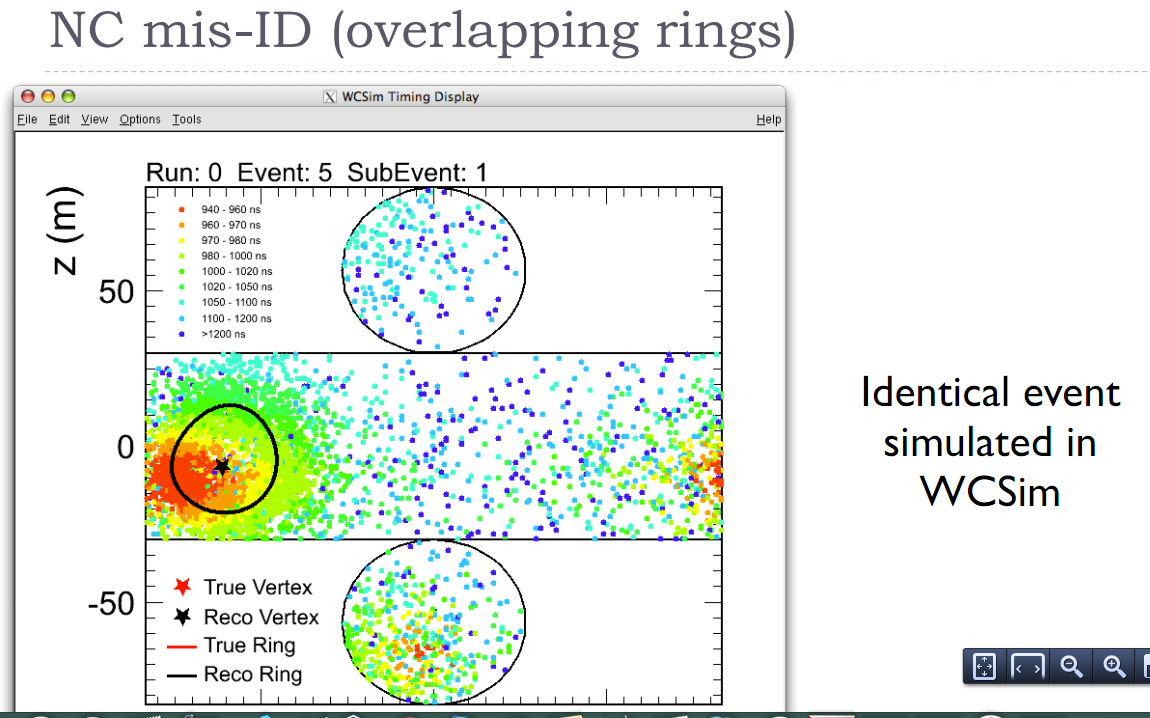
\includegraphics[width=3.0in]{./mtrls/imgs/WCSIM-ovrlap-rings.png}}\\
\subfloat[]{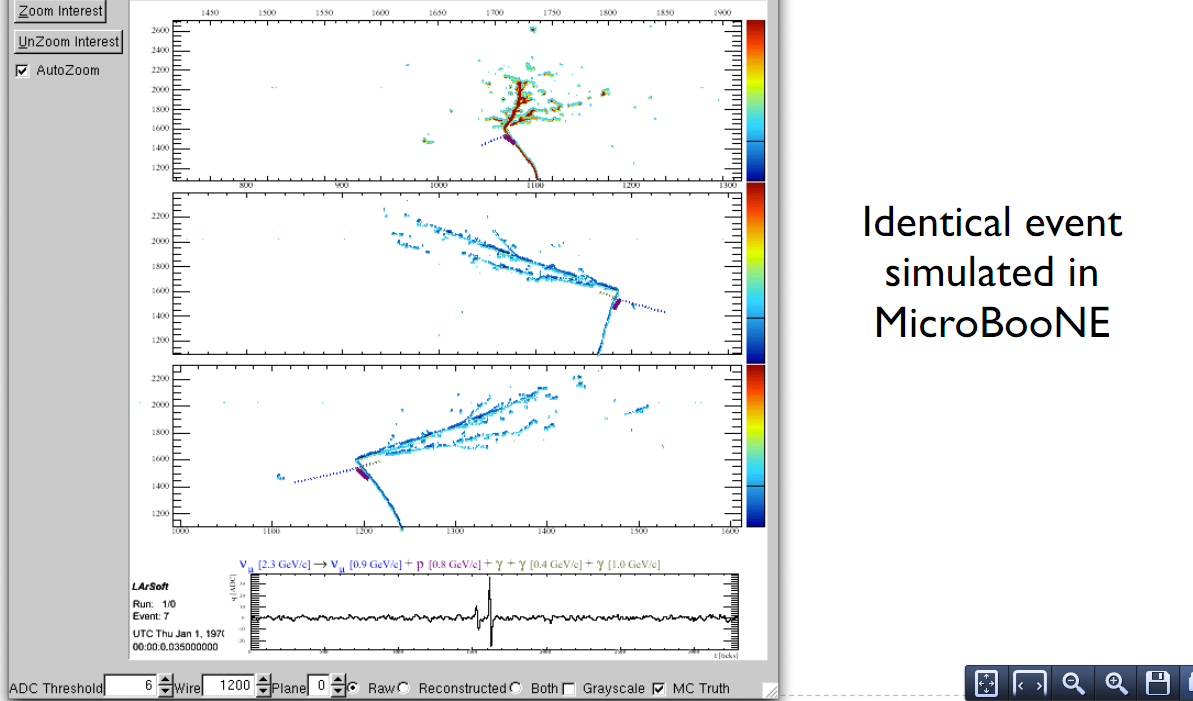
\includegraphics[width=3.0in]{./mtrls/imgs/LAr-uB-ovrlap-rings.png}}%
\label{pi0.overlap}
\end{figure}


\section{Framework and Tools}

BRIAN OUTLINE: Discussion of the fundamentals
- Use of ART
- Availability of hooks for using external packages for event generation, detector simulation
- Requirements for developing a Geometry description
(Ruth -- diagram of modules)


\subsection{ART}
LArSoft is built on the Analysis and Reconstruction Toolkit (ART) framework designed and maintained by the Fermilab Computing Division (CD) for intensity frontier experiments. 
The art framework provides functionality for data transfer, event building, event reconstruction and art analysis framework, process management, system and process state behavior, control messaging, local message logging of status and error messages, DAQ process and art module configuration, and the writing of event data to disk in ROOT format. \cite{art-ref}

Art was chosen because ADD REASON.
\subsection{External Packages}
\subsubsection{Event Generation}
\subsubsection{Detector Simulation}

\subsection{Geometry Description Requirements}
BRIAN:  It should describe the hierarchy of the geometry and how multiple drift volumes, photodetectors, external detectors are handled.  There is no need to list which experiments have geometries, we can list the experiments using LArSoft either in the introduction or in another section.

Figure~\ref{uboone.pic} shows the Geant4 implementation of the MicroBooNE detector geometry in LArSoft.  The top picture shows the entire detector hall region surrounding the cryostat.  The lower left picture shows the interior layout of the active detectors (TPC+PMTs) in the cryostat, and the lower right picture shows details of the TPC.

\hspace*{2cm}
\begin{figure}[h]
\centering
\caption{The LAr40 detector is shown here as built from the gdml scripting language in LArSoft. As specified in the LAr40 design~\cite{lar40CaseStudy} there are 2x3x18 Anode Plane Assemblies shown here in each of two 20 ktonne LAr volumes. Each cryostat is surrounded in rock whose composition is typical of that found at the DUSEL 800 feet level.}
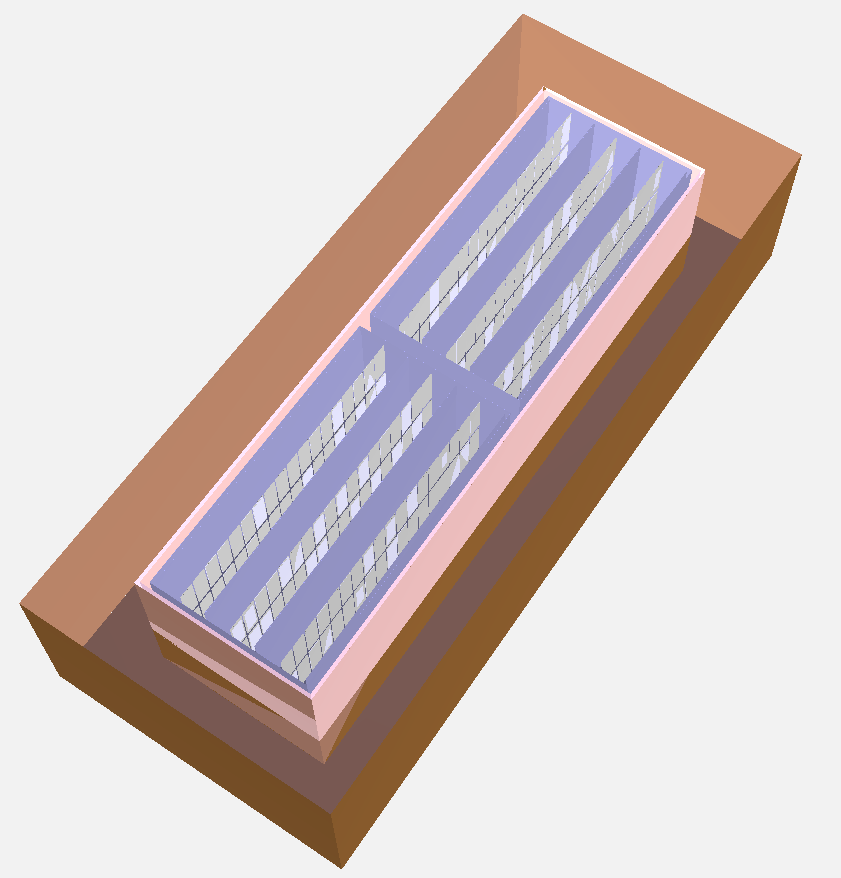
\includegraphics[width=4.0in]{./mtrls/imgs/20111024_lbne_w_APAs2.png}
\label{lar40.img}
\end{figure}

                    
\section{Simulation Mechanics}
BRIAN OUTLINE: 3. Discussion of mechanics for the simulation
- Data product description
- LArSoft specific adaptations for using G4 (the user action lists and readout geometries)
- hooks for adding in additional detectors outside of the LAr volumes
- description of how new parameterizations for ionization, etc can be added into the simulation
- extensions related to incorporating magnetic fields
- Optical simulation

BRIAN: The simulation section should start with an outline along the lines of
1. LArSoft provides interfaces to simulate a variety of interactions and detectors
2.  The simulation is designed for flexibility and does not make assumptions about detector geometry or electronics
3.  Experiments provide the geometry description and electronics simulation


\subsection{Data Product Description}
LArSoft simulation jobs are modular in nature, with each module reading input data objects and writing output data objects to the event.  A typical simulation job is shown in figure~\ref{Fig122}.

As the readout electronics differ for each experiment using LArSoft, each
experiment must provide a detailed simulation of its electronics.  This electronics simulation is currently well-modeled for ArgoNeuT, and is modeled for MicroBooNE with the circuit's LaPlace transform, and a good first approximation place-holder exists for LAr40. 


\subsection{Adaptations for Using G4}
- LArSoft specific adaptations for using G4 (the user action lists and readout geometries)
The truth particles generated in the event generator step are passed to a Geant4 based detector simulation called LArG4.  The geometry GDML file is parsed to create a Geant4 detector description using the built-in GDML parser, which interfaces to LArSoft via the DetectorConstruction LArSoft class.
\subsubsection{User Action Lists}
\subsubsection{Readout Geometries}

\subsection{Adding Additional Detectors}
- hooks for adding in additional detectors outside of the LAr volumes
\subsection{New Parameterizations for Ionization}
- description of how new parameterizations for ionization, etc can be added into the simulation

BRIAN: It should include a description of the mechanism for calculating the amount of ionization charge and scintillation light.  It could include a statement of the available options for that calculation (NEST vs decoupled charge and light) and how a user might add a new method.

\subsection{Incorporating Magnetic Fields}
- extensions related to incorporating magnetic fields
\subsection{Optical Simulation}
BRIAN: describe the basics of how the photon propagation is handled, how electronics are to be simulated for the photodetectors, and how a user could add a photodetector to an experiment.  The details of how each experiment detect photons is not super relevant in this document.

Optical physics simulations in LArSoft can take one of two forms: full or fast 
simulation.  The full simulation involves stepping every optical photon individually through the detector volume.  Typical photon yields for an event can be in the $10^{meh}$ range, hence this is a computationally intensive procedure.  The OpticalPhysics physics constructor has been specially adapted for LArSoft and includes scintillation and Cerenkov production, Rayleigh scattering, reflections at boundaries, absorption at boundaries and in the bulk, and wavelength shifting physics processes.  The configurations of these are described below.

Scintillation production is configured with a photon momentum spectrum of 9.7 ?? 1 eV and a yield of 24,000 photons per MeV of energy loss, incorporating both a fast and a slow component, which can be scaled by a quenching factor specified for each scintillating particle.  These quenching factors, and the possibility of utilizing a more systematic specification of the quenching per particle, require further investigation. Cerenkov photons are produced with yields and energies corresponding to the standard Frank-Tamm spectrum of Cerenkov radiation.\
\
Rayleigh scattering and photon-absorption process are enabled, where the scattering length is specified at 90 cm for all wavelengths and the absorption length is set to 2000 m (approximately infinite) for all wavelengths, for the purposes of preliminary studies.  The vast majority of photons produced are 128-nm scintillation photons, so we do not expect neglecting the wavelength dependence of these parameters to cause a significant problem.\
\
A simplified reflectivity model is used, whereby each type of boundary in the detector is supplied with a wavelength dependent total reflectivity and specular/diffuse reflection fraction.   For  preliminary  studies  only the  steel/argon boundaries  at  the  edge of the cryostat are  reflective,  with  all  other  surfaces,  including  wires,  field cage,  etc,  being opaque.   The steel/argon boundaries have a total reflectance of 25 %, of which 50% is specular.  

\subsubsection{Fast Optical Simulation Modules}

BRIAN: This section can probably be rescued.

Since the stepping of every photon generated in an event is a computationally intensive process, an alternative, fast library sampling simulation is described below.

The optical fiducial volume is divided into optical voxels, and the scintillation light production intensity and time profile in each voxel is recorded.  The sensitive detector configuration is somewhat different to that applied to the charge voxels, since the isotropic light production is a result of a very specific physics process. We can improve efficiency by not requiring stepping particles to know about the presence of optical voxels, but rather supply a modified scintillation process that fills the PhotonVoxelList with the map of scintillation photon production across the detector volume.  The photon voxels are defined separately to charge voxels, since they will undergo a separate size optimization.

A separate module contains a set of PMTHitCollections
 giving the expected final 4-positions and 4-momenta of detected photons for a very intense light source at each voxel in the detector.  By comparing the intensity of the scintillation light source present in each voxel in the event to the intensity of the light sources used to generate the library file, and then applying Poisson fluctuations, a number of photons to sample for each PMT in the geometry is calculated.  A set of photons are sampled from the library file, their detection time is smeared by the time profile of scintillation in each voxel, and by combining the expected responses from the light in each voxel, a PMTHitCollection is generated representing the expected detector response for the event.

The photon library is both geometry and voxelization scheme specific, and changes to either require a full regeneration of the library, which is a one-time computationally intensive job.  The LightSource event generator supplies the intense sources of 9.7 eV photons for library generation, and all optical photons are stepped using the full optical physics simulation. The PMTHitCollections produced by LArG4 for light sources placed in each voxel, as well as the light source intensity, are stored in the library file using a module which is a part of the PhotonPropagation package.  The library building and sampling simulation chain are shown in~\ref{Fig124}.
\hspace{5cm}                         





\section{Reconstruction Mechanics}

BRIAN OUTLINE: 4. Discussion of the reconstruction mechanics
- Data product description
- How the algorithms are organized
- Plan for implementing algorithms and modules
- Mention of anything that is unique to LArSoft (i.e., it isn?t important that we have a Kalman Filter because every tracking experiment implements one)

\subsection{Data Product Description}
\subsection{Organization of Algorithms}
\subsection{Implementation Plan for Algorithms and Modules}
\subsection{Unique aspects of LArSoft Reconstruction}

KEEP OR NOT?
LArSoft contains an event display to understand neutrino events in liquid argon. Reconstruction objects and raw information may be added and removed. Events can be specified for viewing with MC truth info overlaid, if applicable. Zooming features allow insight into the tiniest features around vertices.

The display has been tested with Monte Carlo and ArgoNeuT data, and the code has been written with ease of generalization to MicroBooNE and LAr40 in mind.  

Figure~\ref{argo.evd} shows an example event display for an ArgoNeuT data event.

\hspace*{2cm}
\begin{figure}[h]
\centering
\caption{A data event in ArgoNeuT, viewed with the event display in LArSoft. Among other emitted particles, two $\pi^0$s are evident.}
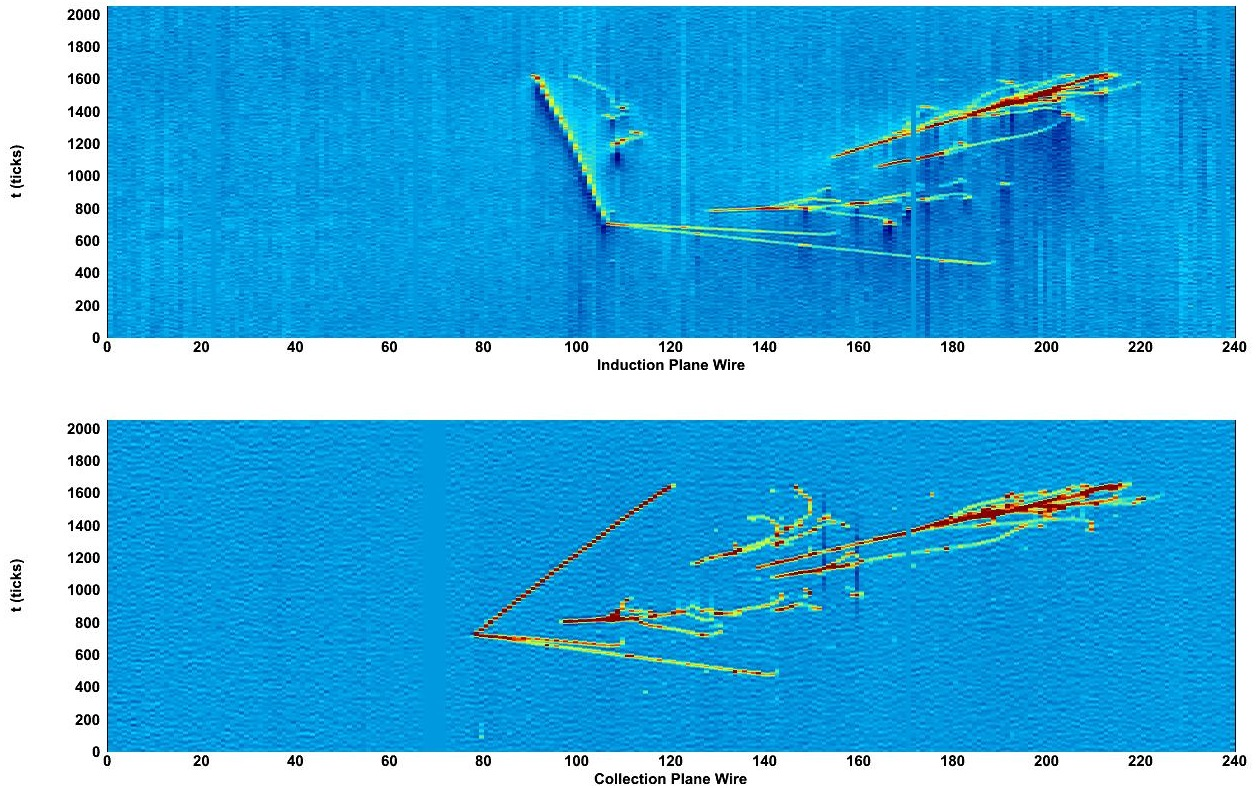
\includegraphics[width=4.0in]{./mtrls/imgs/ArgoNeuT_event.jpg}
\label{argo.evd}
\end{figure}



CAN ANY OF THE FOLLOWING BE KEPT?
LArSoft  benefits from the experience of multiple experiments.  Each LArTPC provides essentially the same basic information after accounting for small detector differences.  Thus, algorithms developed for one experiment can be directly used by another, as long as the differences in geometry are properly accounted for in the algorithms.  The reconstruction chain proceeds in the following steps
\begin{enumerate}
\item First, the raw energy depositions (digits) are calibrated into signals on wires.
\item Next, hits are formed from the regions containing wire signals that are above a tunable threshold.
\item Hits are then grouped into clusters.
\item Clusters are classified to be projections from either 3D tracks or showers. Tracks and showers inherit from the class prong, in the usual C++ sense.
\item Vertices are located using prongs that are shown to originate from a common point.
\item Finally, prongs and vertices are associated into events.
\end{enumerate}
The LArSoft reconstruction chain is complete in that initial algorithms for each step currently exist.  More effort will be required to demonstrate that every, or at least most of the desired, event topologies can be handled in an automated way in the reconstruction chain. Detailed studies of various event classes are in progress to understand the performance of each reconstruction algorithm.

The reconstruction algorithms in LArSoft have benefited from several advances in image analysis techniques developed over the past decade.  For example, the algorithm used to cluster groups of energy depositions together is directly taken from the heavily-cited work of Ester, Kriegel, Sander, and Xu's~\cite{} Density Based Spatial Clustering of Applications with Noise (DBSCAN). The two-dimensional (2D) vertex, or more accurately line-endpoint, finding algorithms are based on a corner finding technique used for locating edges and corners in photographic images.  Initial particle tracking is performed using Hough line finding techniques.

\hspace*{2cm}
\begin{figure}[h]
\centering
\caption{This flow chart shows the objects created along the reconstruction chain in LArSoft.}
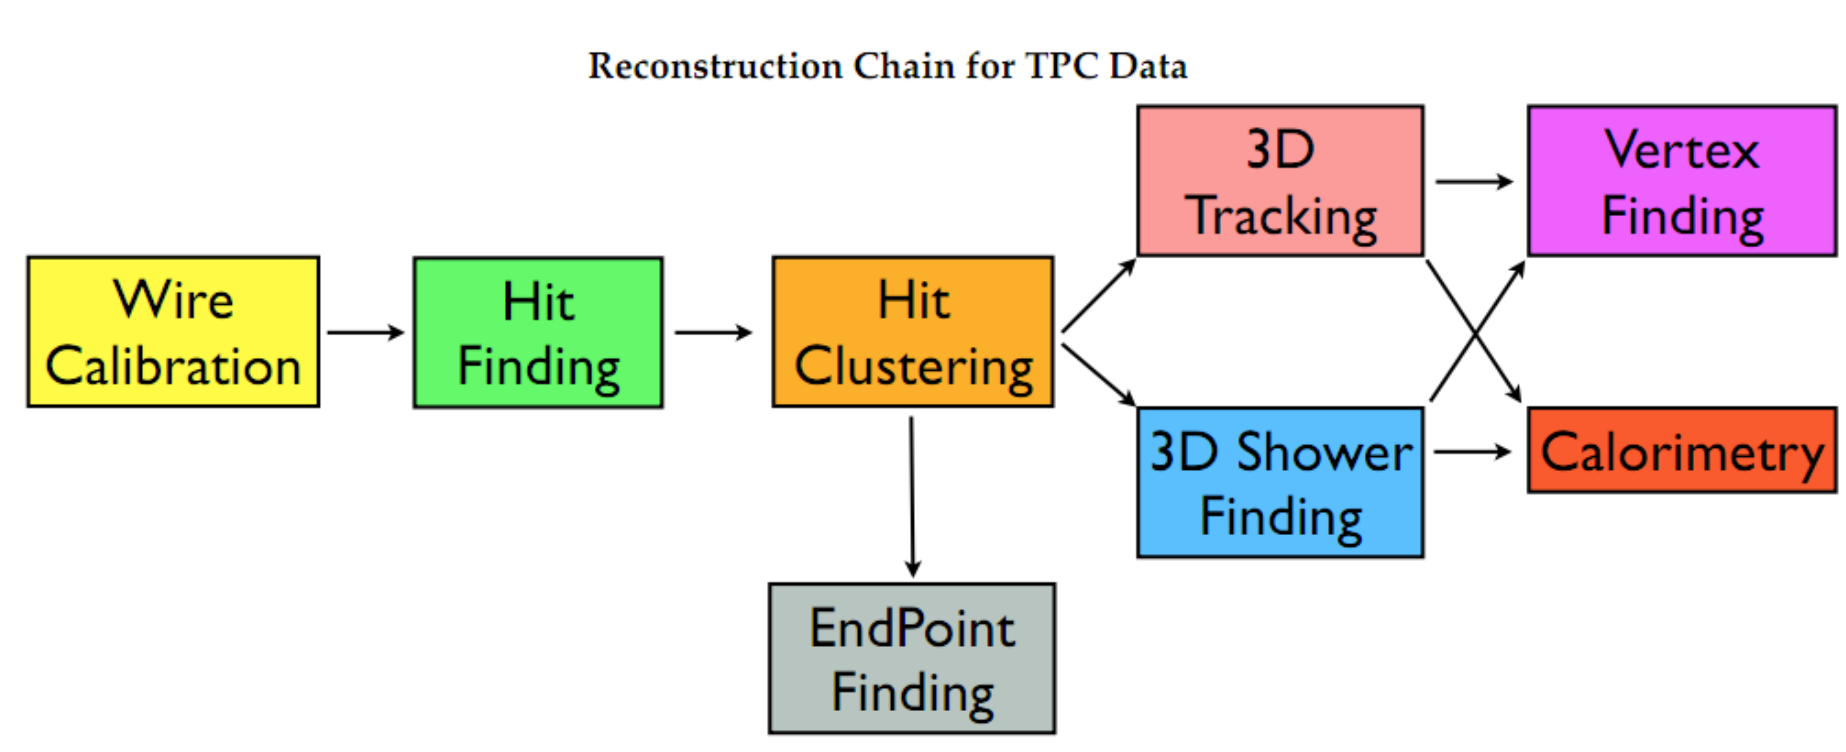
\includegraphics[width=4.0in]{./LArSoft-Recon-Flow-Soderberg.pdf}
\label{flow}
\end{figure}

Tracks, showers, and vertices are three-dimensional (3D) objects. At step 4 above, one begins to need to use the information from the 2D wire plane projections to reconstruct the 3D object from which it originates. Currently the 2D reconstruction codes are robust; the 3D versions are less mature. The following sections summarize the current state of the most important components of the reconstruction code.


Figure~\ref{Fig125} gives an indication of the current capabilities of LArSoft using real data from ArgoNeut. Figure 126 and Figure 127 show an example of a fully reconstructed simulated event using the MicroBooNE implementation of LArSoft.

               
\section{Analysis Mechanics}

BRIAN OUTLINE: Discussion of the analysis mechanics
- Data product description
- How the algorithms are organized
- Plane for implementing algorithms and modules
- Mention of anything that is unique to LArSoft 
\subsection{Data Product Description}
\subsection{Organization of Algorithms for Analysis}
\subsection{Implementation Plan}
\subsection{Unique Analysis Aspects of LArSoft}

\section{Getting Software and Benchmarking it}

BRIAN OUTLINE: (New section) Discussion of how to get the software and benchmarking of it
- How folks can contribute, what the mechanism is for vetting code to go into a release
- Unit testing structure and expectations
- Results for typical memory and CPU usage
\subsection{Ways to Contribute}
Include how to vet code going into a release.

LArSoft is hosted in GIT repositories with ten repositories containing general software, and experiment-specific repositories for digitization code and Configuration files. MultiRepository Build (MRB) compiles code across GIT repositories. Each repository has a test area and some libraries such as EventGenerator, LArG4, HitFinder, VertexFinger, etc.\cite{gian}

Although no one has been identified to vet all code going into a release, there are spot checks and collaboration to enable everyone to be able to contribute to LArSoft. Software that is is violation of the tenants listed at \cite{code tenants} results in discussion with the appropriate experiment spokesperson. Basically, the idea is lean, modular code that is detector agnostic.  

\subsection{Unit Testing}
LArSoft does not run unit tests or regression tests, though modulo manpower has been suggested to the committee.

\subsection{Typical Memory and CPU Usage}

\section{Summary}


\begin{thebibliography}{99}
\bibitem{muboone} http://www-microboone.fnal.gov
\bibitem{gla11}https://www.jyu.fi/fysiikka/en/gla2011/Proceedings
\bibitem{ubtdr}Chapter 12 of MicroBooNE TDR.
\bibitem{t600} S.~Amerio {\it et al.}  ICARUS Collaboration,
  ``Design, construction and tests of the ICARUS T600 detector,''
  Nucl.\ Instrum.\ Meth.\ A {\bf 527}, 329 (2004)]
\bibitem{argo-arxiv} M.~Soderberg {\it et al.}  [ArgoNeuT Collaboration],
  ``Analysis of a Large Sample of Muons with the ArgoNeuT Detector,''
  in preparation.
\bibitem{art-ref} https://cdcvs.fnal.gov/redmine/projects/artdaq
\bibitem{gian} Petrillo, Gianluca, "LArSoft: simulation and reconstruction for Liquid Argon TPC," Liquid Argon TPC R\&D Workshop, Fermilab, July 8, 2014.
\bibitem{codetenants} https://cdcvs.fnal.gov/redmine/projects/larsoft/wiki/The\_rules\_and\_guidelines
\end{thebibliography}
\clearpage 

\tableofcontents

\end{document}







